\documentclass{standalone}
\usepackage{xcolor,amsmath,amssymb,amsfonts}
\usepackage{fontspec}
\usepackage[T1]{fontenc}
\usepackage[tt=false, type1=true]{libertine}
\usepackage[libertine]{newtxmath}

\usepackage{tikz}
\usetikzlibrary{arrows.meta}
\definecolor{red}{HTML}{c63a44}
\begin{document}

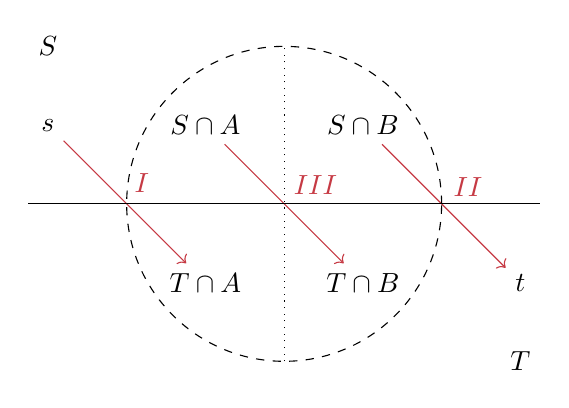
\begin{tikzpicture}
    \node at(-1,-1)(ta){$T\cap A$};
    \node at(-1,1)(sa){$S\cap A$};
    \node at(1,-1)(tb){$T\cap B$};
    \node at(1,1)(sb){$S\cap B$};
    \node at(-3,2){$S$};
    \node at(3,-2){$T$};
    \node at(-3,1)(s){$s$};
    \node at(3,-1)(t){$t$};
    \draw[->,red]
        (s) edge node[above right]{$I$} (ta)
        (sb) edge node[above right]{$II$}(t)
        (sa) edge node[above right]{$III$}(tb);
    \draw[dashed] (0,0) circle (2);
    \draw[dotted] (0,-2) -- (0,2);
    \draw (-3.25,0) -- (3.25,0);
\end{tikzpicture}

\end{document}